\section{ZLP subtraction and bandgap determination in WS$_2$ nanostructures}
\label{sec:results_sample}

Following the discussion of the vacuum results, we now move
to present the application of our fitting strategy to the parametrisation
of EEL spectra recorded on samples.
%
Specifically, we will analyse EELS measurements taken on the WS$_2$ nanostructures
presented in~\cite{SabryaWS2} and reviewed in Sect.~\ref{sec:tmd}.
%
These nanostructures exhibit a flower-like configuration where different layers
of material combine to form the petals and the stem of the flowers.
%
Their geometrical configuration is such that, depending on the specific region
of the nanostructure that one is imaging, the spectra will be sensitive
to different thicknesses and orientations of the material.

The parametrisation of these in-sample EEL spectra will then be used
to subtract the ZLP contribution and extract the bandgap energy $E_{\rm BG}$ from
the behaviour of $I_{\rm inel}(\Delta E)$ in the onset region.
%
The value of the bandgap  has been estimated in different ways
from subtracted EEL spectra, such as by means of the inflection point of the rising intensity or
a linear fit to the maximum positive slope~\cite{Schamm:2003}.
%
Here we will adopt the approach of~\cite{Rafferty:2000} whereby the behaviour
of $I_{\rm inel}(\Delta E)$ in the onset region is  modeled by
\begin{equation}
  \label{eq:I1}
    I_{\rm inel}(\Delta E) \simeq  A \lp \Delta E-E_{\rm BG} \rp^{b} \, , \quad \Delta E \ge E_{\rm BG} \, ,
\end{equation}
and vanishes for $E < E_{\rm BG}$, where $A$ and $b$ are constants extracted from the fit.
%
The power exponent $b$ is expected to be $b\simeq 1/2$ for a semiconductor material characterised
by a direct bandgap, and $b\simeq 3/2$ for the case instead of an indirect bandgap.

\subsection{Training dataset}
%
Fig.~\ref{fig:ws2positions} displays
low-magnification TEM images of two different regions of
the WS$_2$ nanoflowers, denoted as sample A and sample B in the following.
%
In each image we indicate the specific locations where
EEL spectra have been recorded, including in-vacuum measurements taken
for calibration purposes.
%
In the upper image, the differences in contrast are correlated to the material
thickness, with higher contrast corresponding to thinner regions.
%
Here the ZLP parametrisation strategy will be applied separately
to samples A and B, since in each case the EELS measurements have
been obtained with different electron microscopes and
operation settings, which thus as explained in Sect.~\ref{sec:eels}
must be analysed independently.

%%%%%%%%%%%%%%%%%%%%%%%%%%%%%%%%%%%%%%%%%%%%%%%%%%%%%%%%%%%%%%%%%%%%%%%
\begin{figure}[t]
\begin{centering}
  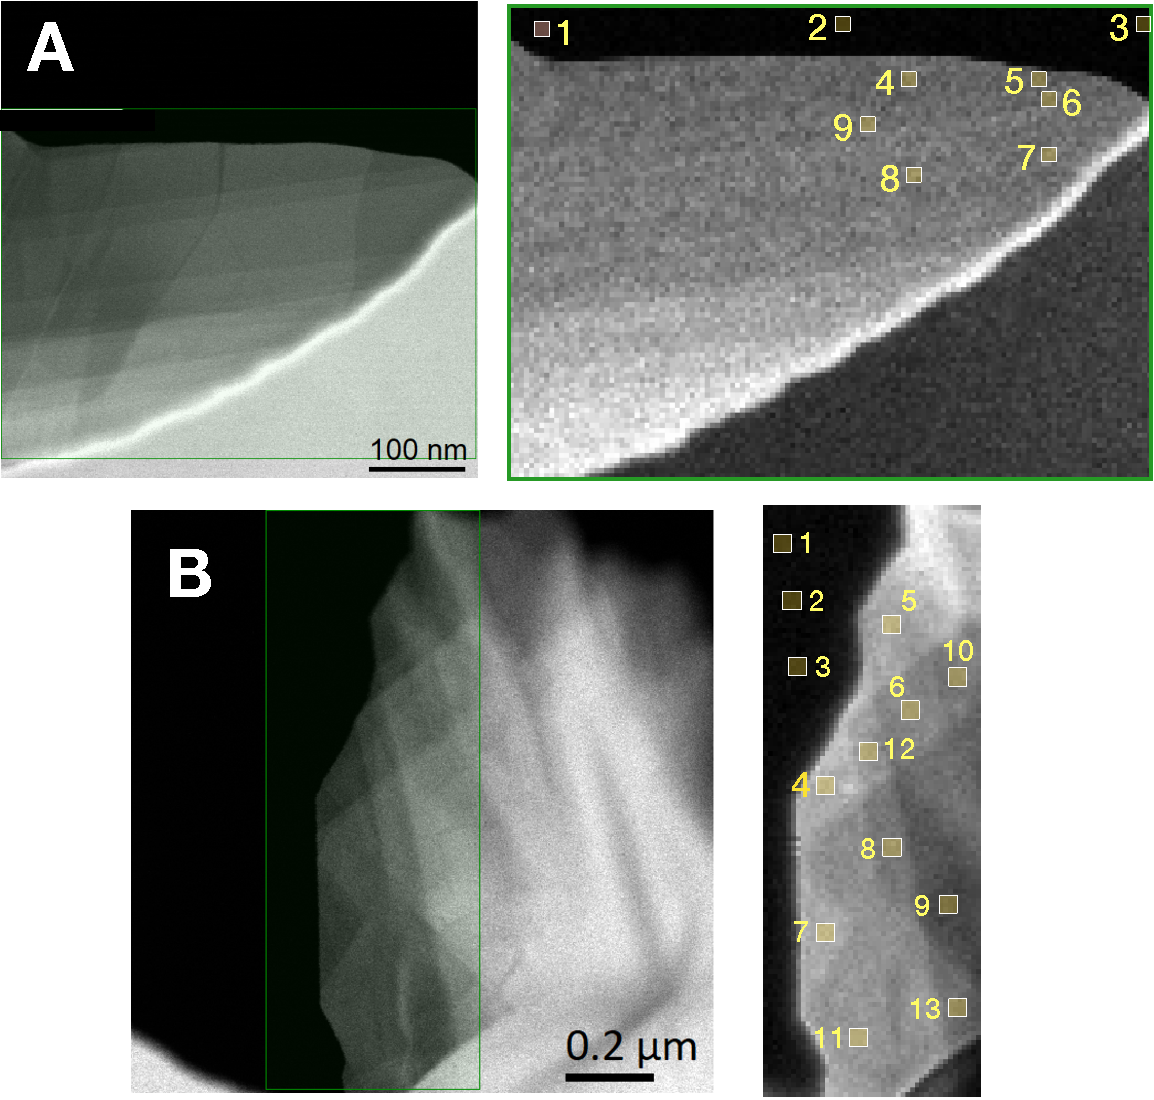
\includegraphics[width=0.87\linewidth]{plots/Spectra_location.pdf}
  \caption{Low-magnification TEM images of two different regions of
    the WS$_2$ nanoflowers, denoted as sample A and sample B respectively.
    %
    In each image we indicate the locations where
    EEL spectra have been recorded, including the in-vacuum measurements taken
    for calibration purposes.
    %
    In sample A the difference in contrast is correlated to the material
    thickness, with higher contrast corresponding to thinner regions of the nanostructure.
  }
\label{fig:ws2positions}
\end{centering}
\end{figure}
%%%%%%%%%%%%%%%%%%%%%%%%%%%%%%%%%%%%%%%%%%%%%%%%%%%%%%%%%%%%%%%%%%%%%%%%%%

In Table~\ref{table:sampledata} we collect the most relevant properties of the spectra collected
in the locations indicated in Fig.~\ref{fig:ws2positions} using the same convention as
in Table~\ref{table:sampledata}.
%
As mentioned, the sets of spectra from samples A and B
have been acquired with different microscopes and thus are
not directly comparable.
%
The full width at half maximum is averaged over all spectra of a given sample,
including those acquired on vacuum.
%
From this table one can observe that ....

%%%%%%%%%%%%%%%%%%%%%%%%%%%%%%%%%%%%%%%%%%%%%%%%%%%%%%%%%%%%%%%%%%%%%%%%%%%%%%%%%%%%%%%%%%%%%
%%%%%%%%%%%%%%%%%%%%%%%%%%%%%%%%%%%%%%%%%%%%%%%%%%%%%%%%%%%%%%%%%%%%%%%%%%%%%%%%%%%%%%%%%%%%%
\begin{table}[t]
  \begin{center}
            \renewcommand{\arraystretch}{1.50}
  \begin{tabular}{@{}ccccccccc}
\br
Set & $t_{\rm exp}$ {(}ms{)} & $E_{\rm b}$ {(}keV{)} & $N_{\rm sp}$ & $N_{\rm dat}$ & $\Delta E_{\rm min}$~(eV)  & $\Delta E_{\rm max}$~(eV)  & FWHM~(eV)  \\ 
\mr
A        &       ?       &    200 keV       &   11     &    2000    &     -0.93        & 9.07   & $\pm$         \\
B        &       ?       &        ?         &   6      &    1918    &     -4.054       & 45.471 & $ \pm$         \\
\br
  \end{tabular}
    \end{center}
  \caption{\small Same as Table~\ref{table:vacuumdata} now for the EEL spectra taken on WS$_2$ nanostructures.
  }
   \label{table:sampledata}
\end{table}
%%%%%%%%%%%%%%%%%%%%%%%%%%%%%%%%%%%%%%%%%%%%%%%%%%%%%%%%%%%%%%%%%%%%%%%%%%%%%%%%%%%%%%%%%%%%%%%%%5
%%%%%%%%%%%%%%%%%%%%%%%%%%%%%%%%%%%%%%%%%%%%%%%%%%%%%%%%%%%%%%%%%%%%%%%%%%%%%%%%%%%%%%%%%%%%%

In the following we will focus on representative spectra, specifically spectra \#4 and \#5 in sample
A and spectra \#14 and \#15 in sample B.
%
The full set of original spectra are made available together with the code used to
analyse them as described in this work, whose installation
and usage instructions are summarised in~\ref{sec:installation}



\subsection{ZLP subtraction}

In Table~\ref{table:sampledata_summary} we display
the mean value and uncertainty of the first local minima, $\Delta E_{\rm min}$,
   averaged over the spectra corresponding to samples A and B from
    Fig.~\ref{fig:ws2positions},
as well as the corresponding values of the hyper-parameters
    $\Delta E_I$ and $\Delta E_{II}$ defined in Fig.~\ref{fig:EELS_toy}.
    %
Recall that as discussed in Sect.~\ref{sec:methodology} only
the data with $\Delta E \le \Delta E_I$ is used for the training
    of the neural network model.
    %
    For $\Delta E \ge \Delta E_{II}$ instead the training set includes only the pseudo-data
    that implements the $I_{\rm ZLP}(\Delta E)\to 0$ constraint.

%%%%%%%%%%%%%%%%%%%%%%%%%%%%%%%%%%%%%%%%%%%%%%%%%%%%%%%%%%%%%%%%%%%%%%%%%%%%%%%%%%%%%%%%%%%%%
%%%%%%%%%%%%%%%%%%%%%%%%%%%%%%%%%%%%%%%%%%%%%%%%%%%%%%%%%%%%%%%%%%%%%%%%%%%%%%%%%%%%%%%%%%%%%
\begin{table}[t]
  \begin{center}
            \renewcommand{\arraystretch}{1.50}
  \begin{tabular}{@{}ccccccccc}
\br
Set & $\Delta E_{\rm min}$~(eV)  &  $\Delta E_I$~(eV)  &  $\Delta E_{II}$~(eV)   \\
\mr
A        &    $\pm$                &                   &              \\
B        &    $\pm$               &                     &               \\
\br
  \end{tabular}
    \end{center}
  \caption{\small The mean value and uncertainty of the first local minima, $\Delta E_{\rm min}$,
    averaged over the spectra corresponding to samples A and B from
    Fig.~\ref{fig:ws2positions}.
    %
    We also indicate
     the corresponding values of the hyper-parameters
     $\Delta E_I$ and $\Delta E_{II}$ defined in Fig.~\ref{fig:EELS_toy} used for the training
     of the neural network model.
    %
  }
   \label{table:sampledata_summary}
\end{table}
%%%%%%%%%%%%%%%%%%%%%%%%%%%%%%%%%%%%%%%%%%%%%%%%%%%%%%%%%%%%%%%%%%%%%%%%%%%%%%%%%%%%%%%%%%%%%%%%%5
%%%%%%%%%%%%%%%%%%%%%%%%%%%%%%%%%%%%%%%%%%%%%%%%%%%%%%%%%%%%%%%%%%%%%%%%%%%%%%%%%%%%%%%%%%%%%

 We find that the location of the first minima is relatively stable
 among all the spectra belonging to given set.
 %
 The neural network training is performed for a wide range of $\Delta E_I$ values
 subject to the condition that $\Delta E_I \le \Delta E_{\rm min} $,
 and the optimal value listed  in Table~\ref{table:sampledata_summary} are selected
 by means of comparing the intensity derivatives in the sample with those
 of the vacuum, as we discuss below.

 Upon completion of the neural network training, one ends up with $N_{\rm rep}=500$ replicas
 of the zero-loss peak associated to each sample, $I_{\rm ZLP}^{({\rm mod})(k)}(\Delta E)$.
 
 Spectra subtracted over replicas

 Matching at very low energy lossess

 Fit procedure over replicas

%%%%%%%%%%%%%%%%%%%%%%%%%%%%%%%%%%%%%%%%%%%%%%%%%%%%%%%%%%%%%%%%%%%%%%%
\begin{figure}[t]
\begin{centering}
  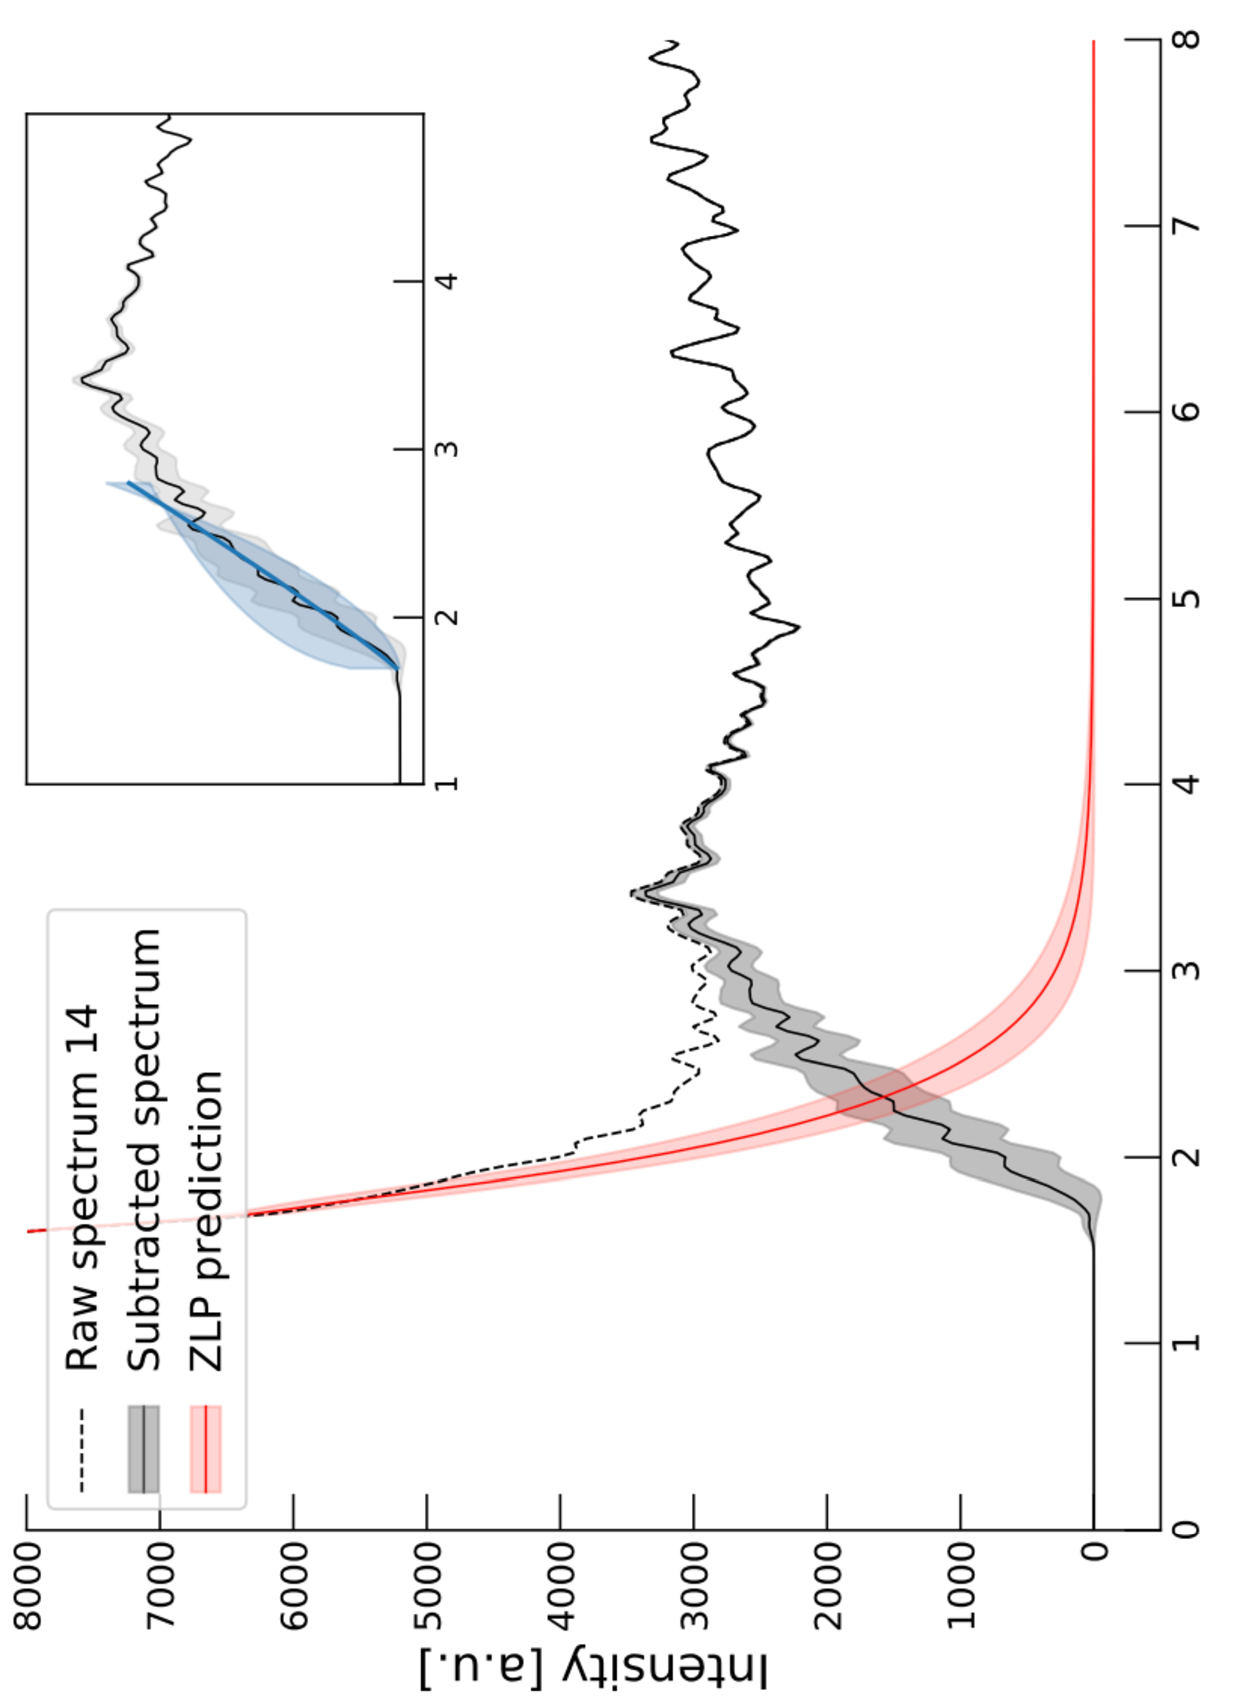
\includegraphics[width=0.36\linewidth,angle=-90]{plots/sp4_subtracted_spectrum.pdf}
   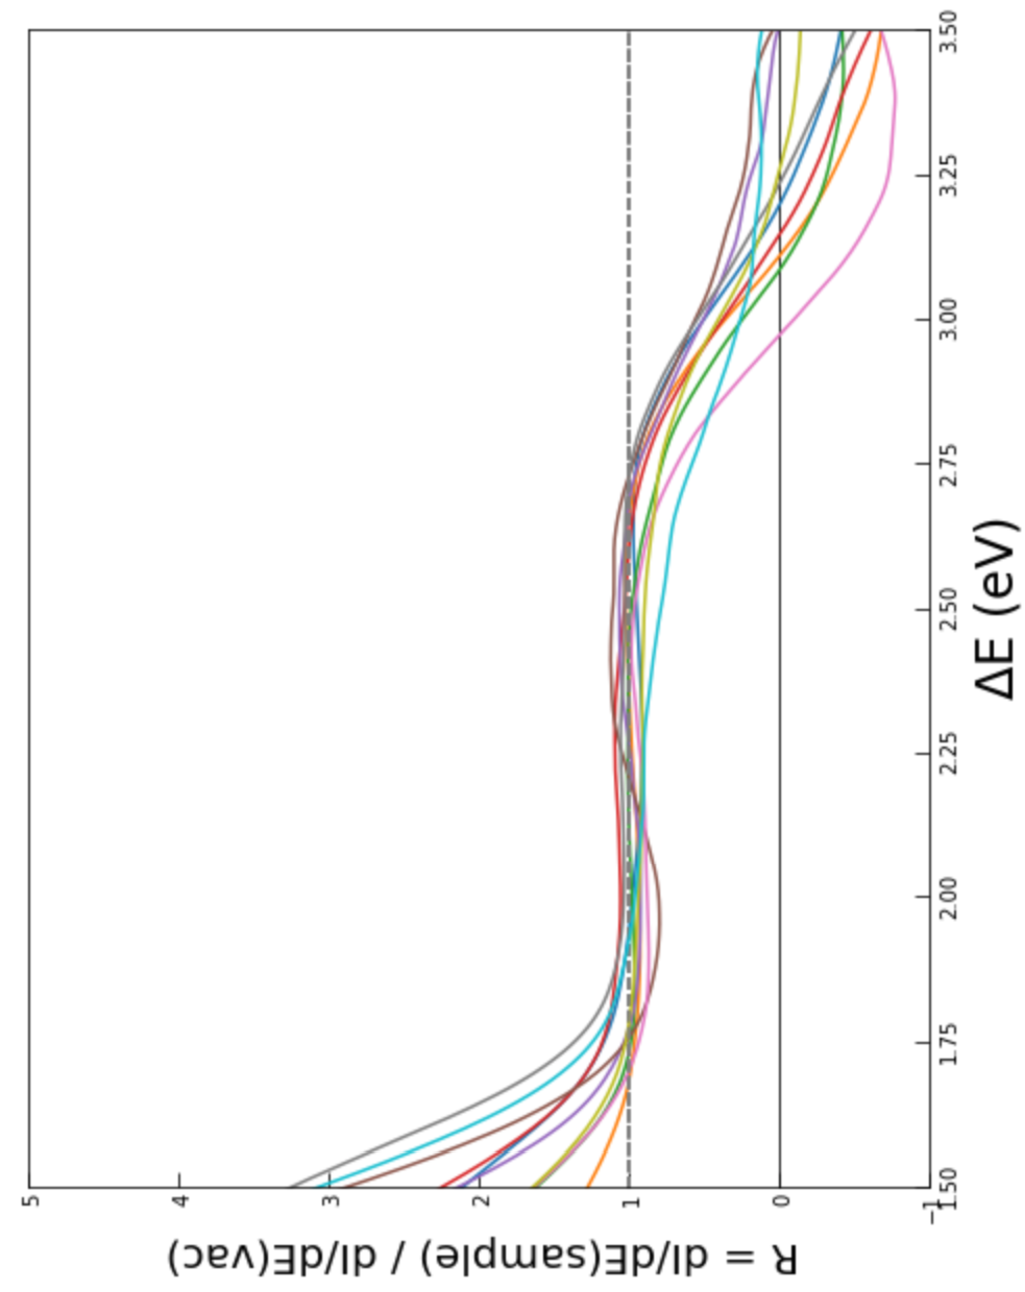
\includegraphics[width=0.36\linewidth,angle=-90]{plots/derivatives.pdf}
   \caption{Left: the original
     and subtracted EEL spectrum corresponding to location \#4 in Fig.~\ref{fig:ws2positions},
     together with the predictions of the ZLP models.
     %
     The inset displays the result of the parabolic fit using Eq.~\ref{eq:I1} to the onset
     region of the subtracted spectrum.
     %
     Right: The ratio of the derivative intensity of the original spectrum, $dI_{\rm EEL}/d\Delta E$,
     over that of the ZLP measurements taken on the vacuum $d I_{\rm ZLP}/d\Delta E$.
  }
\label{fig:sp4_subtracted_spectrum}
\end{centering}
\end{figure}
%%%%%%%%%%%%%%%%%%%%%%%%%%%%%%%%%%%%%%%%%%%%%%%%%%%%%%%%%%%%%%%%%%%%%%%%%%



%
A collection of electron loss spectra acquired at different positions 
at the specimen is used to construct the neural network training inputs. 
%
These sets of data were obtained directly from~\cite{SabryaWS2}.
%
A specimen image of the positions can be observed in figure~\ref{fig:ws2positions}.  
This nanostructure exhibits flat layers with different thicknesses, which 
can be distinguished from the picture as color differences.
%
Energy loss spectra obtained at positions 1-3 are vacuum recordings, 
positions 4-13 represent in-sample data.
%
One layer (S-W-S) WS$_2$ has a thickness of around 0.9 nm. 
The thickness of the specimen at location 5 is 2.11 nm ($\sim$2 layers).



\subsection{Bandgap determination}

Therefore, the bandgap nature (direct or indirect) can be extracted by 
least-squares fitting of each k-th replica subtracted spectrum to equation~\ref{eq:I1}.
%
By averaging over all replicas, one can determine $\textless{b}\textgreater{}$, 
$\textless{E_{BG}}\textgreater{}$ 
and their uncertainties, while keeping track of how the free parameter
E$_{BG}$ is sensitive to the choice of $\Delta$E$_1$, which marks the onset
of the subtracted spectrum intensity.
%

%

In Fig.~\ref{fig:bvalues} Top: the values of the bandgap energy $E_{\rm BG}$ and of the exponent $b$
  obtained from fits to the onset
  region of subtracted spectra using Eq.~(\ref{eq:I1}) as a function
  of the hyper-parameter $\Delta E_I$.
  %
  We show results for locations \#4 (left)
  and \#5 (right panels) from Sample A indicated in Fig.~\ref{fig:ws2positions}.
  %
  The central value and the error band for each value of $\Delta E_I$ is evaluated
  as the median and the 68\% CL interval over the $N_{\rm rep}=500$ Monte Carlo replicas.

%%%%%%%%%%%%%%%%%%%%%%%%%%%%%%%%%%%%%%%%%%%%%%%%%%%%%%%%%%
\begin{figure}[t]
\begin{centering}
  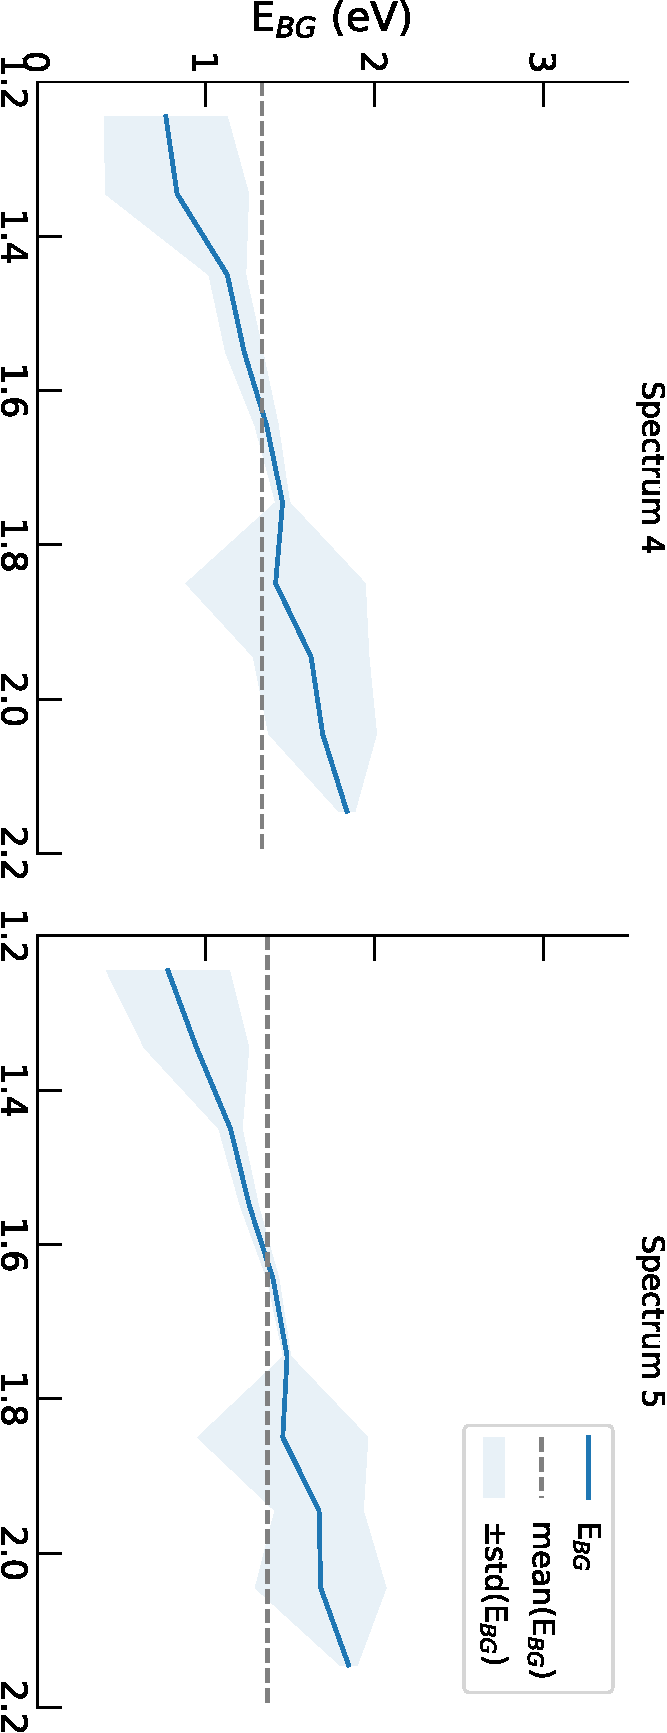
\includegraphics[width=0.38\linewidth,angle=90]{plots/bg_values_sampleA_sp4_sp5.pdf}
  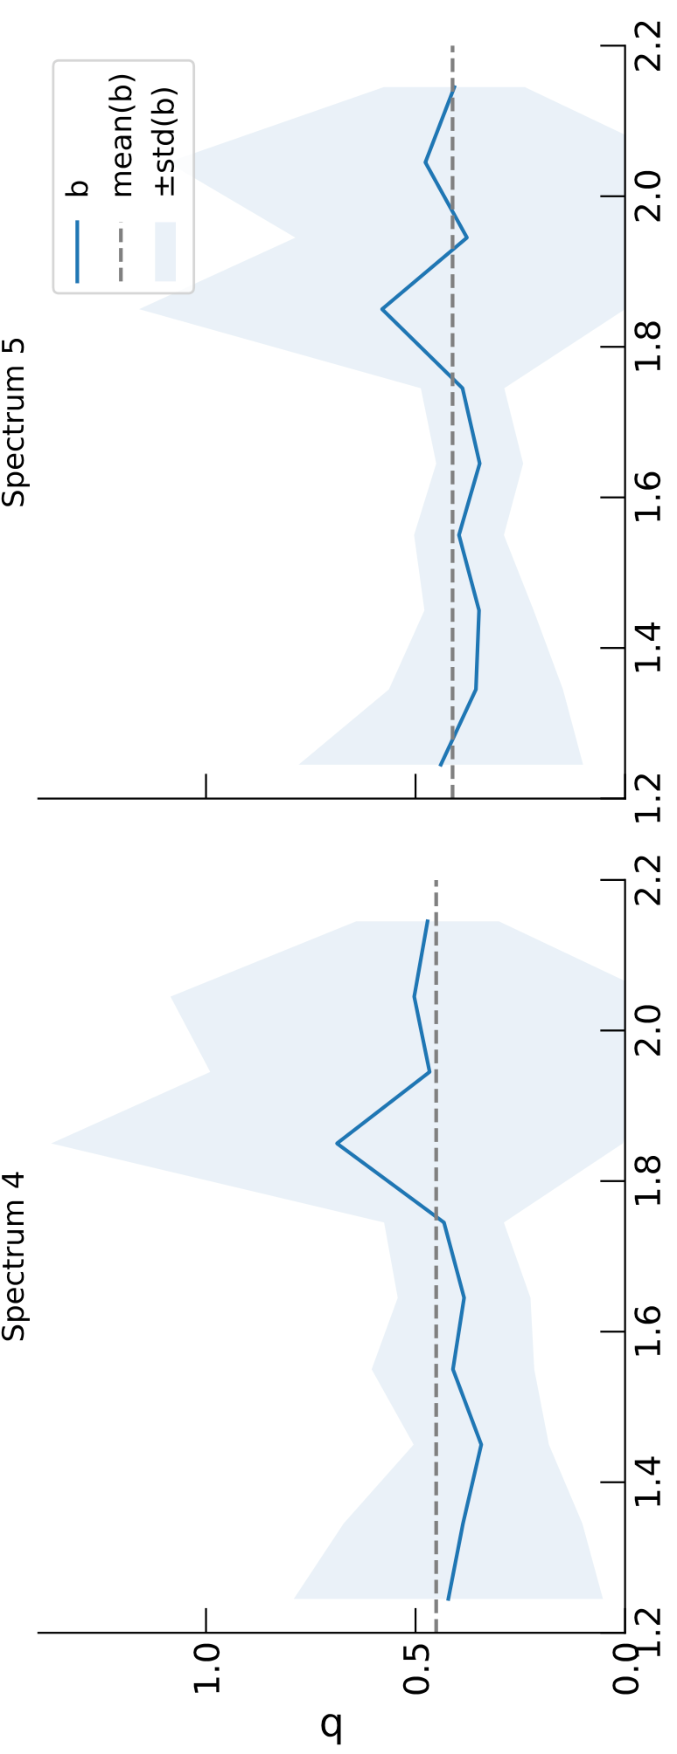
\includegraphics[width=0.38\linewidth,angle=-90]{plots/bvalues_sampleA_sp4_sp5.pdf} 
  \caption{Top: the values of the bandgap energy $E_{\rm BG}$ and of the exponent $b$
  obtained from fits to the onset
  region of subtracted spectra using Eq.~(\ref{eq:I1}) as a function
  of the hyper-parameter $\Delta E_I$.
  %
  We show results for locations \#4 (left)
  and \#5 (right panels) from Sample A indicated in Fig.~\ref{fig:ws2positions}.
  %
  The central value and the error band for each value of $\Delta E_I$ is evaluated
  as the median and the 68\% CL interval over the $N_{\rm rep}=500$ Monte Carlo replicas.
  }
\label{fig:bvalues}
\end{centering}
\end{figure}
%%%%%%%%%%%%%%%%%%%%%%%%%%%%%%%%%%%%%%%%%%%%%%%%%%%%%%%%%%%%%





